\documentclass[main.tex]{subfiles}
\begin{document}
    \chapter{Linear Algebra}
        \label{ch: Linear Algebra}
        \thispagestyle{noheader}

        There is lots of vector maths associated with what is typically Linear Algebra that is used quite often in physics. The relevant maths is covered here, though the topic of Linear Algebra is far more expansive than what is covered here.\\
        Since the most common dimension set dealt with in physics is 3D this shall be what is explicitly covered here. Though it is worth noting that, for the most part, the definitions carry to further dimensions in the way that you would expect.

        \section{Coordinate \& Vector Notation}
            \label{sec: Coordinate and Vector Notation}
            
            \subsection{$\Reals^n$ Notation}
                \label{subsec: Rn Notation}

                This may seem odd at first but this notation is actually pretty simple. Real numbers are numbers with a decimal place (potentially all 0s) and the set of all real numbers is $\Reals$. $\Reals^n$ just means the set of all vectors with $n$ real number components.\\
                There is also the set of all complex numbers $\Complexs$ and $\Complexs^n$ would mean vectors with $n$ complex components.

                Technically $\Reals^n$ is actually something called a \textit{vector space} and has a predefined set of rules, but that's a bit much formal maths for this.

            \subsection{3D Point Notation}
                \label{subsec: 3D Point Notation}

                Points in a 3D system are typically referred two as existing in $\Reals^3$ (they have an $x$, $y$ and $z$ coordinate and each of them is a decimal number / not complex).
                A point is denoted by comma-separated numbers enclosed in round brackets e.g. $(1,\, 2,\, 3)$.

            \subsection{3D Vector Notation}
                \label{subsec: 3D Vector Notation}

                A vector is the same, except a vector ``points'' to a point.
                Vectors are denoted most often using 3 numbers written vertically inside square brackets, though sometimes they may be written inside round brackets, or horizontally like a point except in square brackets. To maintain consistency, only square brackets will be used here to refer to vectors.
                \begin{equation*}
                    \Matrix{x\\y\\z}, \hspace{10mm} \left[x,\, y,\, z\right], \hspace{10mm} \left(\begin{matrix}
                        x\\y\\z
                    \end{matrix}\right)
                \end{equation*}
            
                A vector can also be represented algebraically using an arrow, a harpoon, a squiggle underneath, or even in bold.
                \begin{equation*}
                    \vec{v}, \hspace{10mm} \hvec{v}, \hspace{10mm} \svec{v}, \hspace{10mm} \bvec{v}
                \end{equation*}
                
                \newpage
                This is not to say that the vector cannot be written in component form, this is just a simplified way of representing it. They are often written this way to reduce the amount of working needed.
                \begin{equation*}
                    \vect{v} = \Matrix{v_x\\v_y\\v_z}
                \end{equation*}



            \subsection{The Zero Vector}
                \label{subsec: The Zero Vector}

                The zero vector is denoted by $\vect{0}$ and represents the vector of all zeros.
                \begin{equation}
                    \vect{0} = \Matrix{0\\0\\0}
                \end{equation}



            \subsection{Vectors Between Points}
                \label{subsec: Vectors Between Points}

                Let's say you have two points $A$ and $B$ and you want to draw a vector that points from point $A$ to point $B$. To denote this you simply write $\lhvec{AB}$.\\
                Let's also say that the points have vectors pointing to them $\vect{a}$ and $\vect{b}$.

                \begin{equation*}
                    \vect{a} = \Matrix{A_x\\A_y}
                \end{equation*}
                \begin{equation*}
                    \vect{b} = \Matrix{B_x\\B_y}
                \end{equation*}

                To calculate what this vector is, we do $final - initial$ and, since this vector starts at $A$ and ends at $B$, we get \eqref{eq: Final-Intial Vector}\\
                (See \secref{subsec: Vector Addition and Subtraction} for more information on vector subtraction)

                \begin{equation}
                    \lhvec{AB} = final - initial = \vect{a} - \vect{b}
                    \label{eq: Final-Intial Vector}
                \end{equation}

                The cool thing about vectors is that they point at something, but they do not have a fixed starting point, in some sense they are free to float around the coordinates so long as they still have the same components.

                This can be seen in \figref{fig: Vector Between Points}

                \begin{figure}[!h]
                    \centering
                    \begin{subfigure}[t]{0.45\textwidth}
                        \centering
                        \scalebox{0.8}
                        {
                            %trims left, bottom, right, top
                        \begin{adjustbox}{clip,trim=35mm 10mm 20mm 10mm}
                            {\import{images}{Vector Between Points Fixed.pgf}}
                        \end{adjustbox}
                        }
                    \end{subfigure}
                    \hfill
                    \begin{subfigure}[t]{0.45\textwidth}
                        \centering
                        \scalebox{0.8}
                        {
                            %trims left, bottom, right, top
                        \begin{adjustbox}{clip,trim=35mm 10mm 15mm 10mm}
                            {\import{images}{Vector Between Points Floating.pgf}}
                        \end{adjustbox}
                        }
                    \end{subfigure}
                    \vspace{-5mm}
                    \caption{Diagrams showing the vector between points $A$ and $B$.}
                    \label{fig: Vector Between Points}
                \end{figure}

                It might now also be more obvious that when we talk about a vector $\vect{a}$ we are also essentially talking about a vector pointing to the point $A$ from the origin. So the final point is $V$ and the initial is $0$
                \begin{equation}
                    \vect{a} = final - initial = \vect{a} - \vect{0}
                \end{equation}

                \newpage




        \section{Vector Operations}
            \label{sec: Vector Operations}

            \subsection{Scalar Multiplication}
                \label{subsec: Scalar Multiplication}

                Vectors can be multiplied by a real scalar (a number) such that \eqref{eq: vector scalar multiplication} is satisfied.
                \begin{equation}
                    \gamma \vect{v} = \gamma \Matrix{v_x\\v_y\\v_z} \deq \Matrix{\gamma v_x\\ \gamma v_y\\ \gamma v_z}, \hspace{5mm} \gamma \in \Reals
                    \label{eq: vector scalar multiplication}
                \end{equation}
                (Dividing is also fine since you could write $\gamma = \frac{1}{2}$)

                \subsubsection{Properties of Scalar Multiplication}
                    \label{subsubsec: Properties of Scalar Multiplication}

                    Scalar multiplication is distributive with addition.
                    \begin{equation}
                        (\gamma + \mu)\vect{v} = \gamma \vect{v} + \mu \vect{v}
                    \end{equation}
                    

                    The order that you multiply also doesn't matter.
                    \begin{equation}
                        \gamma(\mu \vect{v}) = (\gamma \mu)\vect{v}
                    \end{equation}





            \subsection{Addition \& Subtraction}
                \label{subsec: Vector Addition and Subtraction}

                Vectors can be added and subtracted e.g. $\vect{v} + \vect{u}$ or $\vect{v} - \vect{u}$ and this is represented component-wise as 
                \begin{equation}
                    \vect{v} + \vect{u} = \Matrix{v_x\\v_y\\v_z} + \Matrix{u_x\\u_y\\u_z} \deq \Matrix{v_x + u_x\\v_y + u_y\\v_z + u_z}
                \end{equation}
                Subtraction can also be thought of as adding the negative of another vector i.e. $\vect{v} - \vect{u} = \vect{v} + (-\vect{u})$
                
                \subsubsection{Properties of Addition}
                    \label{subsubsec: Properties of Addition}
                    Addition is what is called commutative (order doesn't matter). Subtraction is not though.
                    \begin{equation}
                        \vect{v} + \vect{u} = \vect{u} + \vect{v}
                    \end{equation}
                    \begin{equation}
                        \vect{v} - \vect{u} = -\vect{u} + \vect{v}
                    \end{equation}
                    Addition of vectors is what we call associative, just like normal addition (i.e. the order of bracket operations doesn't matter).
                    \begin{equation}
                        \vect{a} + (\vect{b} + \vect{c}) = (\vect{a} + \vect{b}) + \vect{c}
                        \label{eq: Associativity of Vector Addition}
                    \end{equation}
                    Subtraction is as well, as long as you group the negative sign with the vector.
                    \begin{equation}
                        \vect{a} + (\vect{b} - \vect{c}) = (\vect{a} + \vect{b}) - \vect{c} = -\vect{c} + (\vect{a} + \vect{b})
                    \end{equation}
                    

                    Scalar multiplication is distributive across addition (it works like normal expanding).
                    \begin{equation}
                        \gamma(\vect{v} + \vect{u}) = \gamma \vect{v} + \gamma \vect{u}
                    \end{equation}


                \subsubsection{Adding Vectors Visually}
                    \label{subsubsec: Adding Vectors Visually}

                    It is also possible to perform component-wise addition and subtraction with vectors visually.\\
                    To add two vectors simply place the tail of one vector on the tip of the other vector. For instance, with $\vect{a} + \vect{b}$ you could move $\vect{b}$ so that its tail is on the tip of $\vect{a}$. The important step is that the first vector must have its tail on the origin.

                    You can perform subtraction this way but you must also remember that the order matters with subtraction. The way to get around this is to add the negative version of the vectors (and since order doesn't matter with addition you can then do this in any order).

                    \begin{figure}[!h]
                        \centering
                        \begin{subfigure}[t]{0.45\textwidth}
                            \centering
                            \scalebox{0.8}
                            {
                                %trims left, bottom, right, top
                            \begin{adjustbox}{clip,trim=35mm 10mm 15mm 10mm}
                                {\import{images}{Vector Addition Diagram.pgf}}
                            \end{adjustbox}
                            }
                        \end{subfigure}
                        \hspace{2em}
                        \begin{subfigure}[t]{0.45\textwidth}
                            \centering
                            \scalebox{0.8}
                            {
                                %trims left, bottom, right, top
                            \begin{adjustbox}{clip,trim=35mm 10mm 15mm 10mm}
                                {\import{images}{Vector Subtraction Diagram.pgf}}
                            \end{adjustbox}
                            }
                        \end{subfigure}
                        \vspace{-5mm}
                        \caption{Diagrams showing visual vector addition and subtraction of vectors $\bvec{a}$ and $\bvec{b}$.}
                        \label{fig: Visual Vector Addition}
                    \end{figure}


            \newpage

            \subsection{Modulus}
                \label{subsec: Modulus}

                Vectors are said to have ``magnitude and direction'' since they point somewhere and have a length. The modulus of a vector returns this size. For 2D and 3D it is derived from  pythagoras' theorem which gives the length of the hypotenuse, though for higher dimensions it is assumed that the formula continues to work.
                It is denoted by either one or two sets of absolute value signs.
                \begin{equation*}
                    \left\|\vect{v}\right\|, \hspace{10mm} |\vect{v}|
                \end{equation*}
                Sometimes, if there is a vector such as radial position $\vect{r}$, the modulus will just be denoted without the arrow i.e. $r$ (though this is really a definition of $\vmod{\vect{r}}=r$).
                \vspace{1em}
                
                The modulus function is defined in \eqref{eq: Vector Modulus Definition}
                \begin{equation}
                    \vmod{\vect{v}} \deq \sqrt{v_x^2 + v_y^2 + v_z^2}
                    \label{eq: Vector Modulus Definition}
                \end{equation}
                For vectors in $\Reals^n$, this is defined by \eqref{eq: Modulus Rn}
                \begin{equation}
                    \vmod{\vect{v}} \deq \sqrt{\sum_{i=1}^n v_i^2}
                    \label{eq: Modulus Rn}
                \end{equation}

                \subsubsection{Properties of Modulus}
                    \label{subsubsec: Properties of Modulus}

                    It is important to be careful when using modulus, as modulus does not carry through calculations as one might initially expect. It should be obvious when considering the formula that these properties are true, but it is still good to be careful.
                    \begin{equation}
                        \vmod{\gamma \vect{v}} = |\gamma| \vmod{\vect{v}}
                    \end{equation}
                    \begin{equation}
                        \vmod{\vect{v} + \vect{u}} = \vmod{\vect{v}} + \vmod{\vect{u}} : \, \vect{u} = \gamma \vect{v}
                        \label{eq: Modulus Addition Inequality}
                    \end{equation}

                    \eqref{eq: Modulus Addition Inequality} highlights the fact that modulus is only additive if two vectors are scalar multiples of each other.

                    




            \subsection{Unit Vectors}
                \label{subsec: Unit Vectors}

                Unit vectors are vectors with a \textit{unit} length (1). In that sense they have only a direction. In physics this is even more true since a unit vector also has no dimension, because it is defined as being divided by its own length (\eqref{eq: Unit Vector Definition}). A unit vector is denoted with a ``hat'' above the vector symbol when written algebraically i.e. $\vhat{v}$.

                \begin{equation}
                    \vhat{v} \deq \left\{\begin{array}{cr}
                        \vect{0} & \vmod{\vect{v}} = 0\vspace{3mm}\\ 
                        \bfrac{\vect{v}}{\vmod{\vect{v}}} & \vmod{\vect{v}} \neq 0\\
                    \end{array}\right.
                    \label{eq: Unit Vector Definition}
                \end{equation}
                

                If the vector is not the zero vector, then the length is always 1.
                \begin{equation}
                    \vmod{\vhat{v}} = 1
                \end{equation}




            
            \newpage
            \subsection{The Dot Product}
                \label{subsubsec: The Dot Product}

                The dot product (sometimes called the scalar product) of two vectors is written as $\vect{v} \cdot \vect{u}$.\\
                It produces a scalar result and the definition is given in \eqref{eq: vector dot product}.
                \begin{equation}
                    \vect{v} \cdot \vect{u} = \Matrix{v_x\\v_y\\v_z} \cdot \Matrix{u_x\\u_y\\u_z} \deq v_x u_x + v_y u_y + v_z u_z
                    \label{eq: vector dot product}
                \end{equation}
                In $\Reals^n$ this is defined by \eqref{eq: Dot Product Rn}
                \begin{equation}
                    \vect{v} \cdot \vect{u} \deq \sum_{i=1}^n v_i u_i
                    \label{eq: Dot Product Rn}
                \end{equation}

                The dot product is also related to trigonometry by the identity in \eqref{eq: dot product cos identity}
                \begin{equation}
                    \vect{v} \cdot \vect{u} = \vmod{\vect{v}} \vmod{\vect{u}} \cos\theta
                    \label{eq: dot product cos identity}
                \end{equation}
                Where $\theta$ is the angle between the two vectors.\\
                In this equation it should be clear that the dot product also measures how parallel two vectors are, as when the vectors are completely parallel then $\cos\theta = 1$ and if they are perpendicular then $\cos\theta = 0$.

                \begin{figure}[!h]
                    \centering
                    \scalebox{0.7}
                    {
                        %trims left, bottom, right, top
                        \begin{adjustbox}{clip,trim=10mm 5mm 10mm 10mm}
                            {\import{images}{2D Vector Diagram.pgf}}
                        \end{adjustbox}
                    }
                    \vspace{-8mm}
                    \caption{A diagram showing two vectors $\bvec{v}$ and $\bvec{u}$, and the angle between them.}
                    \label{fig: Dot Product Diagram}
                \end{figure}
            
                \subsubsection{Properties of the Dot Product}
                    \label{subsubsec: Properties of the Dot Product}

                    The dot product still obeys most of the standard rules of multiplication.
                    \begin{equation}
                        \vect{v} \cdot \vect{u} = \vect{u} \cdot \vect{v}
                    \end{equation}
                    \begin{equation}
                        \gamma(\vect{v} \cdot \vect{u}) = (\gamma \vect{v}) \cdot \vect{u} = \vect{v} \cdot (\gamma\vect{u})
                    \end{equation}
                    \begin{equation}
                        \vect{a} \cdot (\vect{b} + \vect{c}) = \vect{a} \cdot \vect{b} + \vect{a} \cdot \vect{c}
                    \end{equation}

                    It also gives the vector modulus.
                    \begin{equation}
                        \vect{v} \cdot \vect{v} = \vmod{\vect{v}}^2
                    \end{equation}
            
            \newpage
            \subsection{The Cross Product}
                \label{subsubsec: The Cross Product}

                The cross product is more complicated and the formula can be a little more confusing so, if you aren't too sure what's going on, don't worry yet.\\
                The cross product takes two vectors and considers how \textit{orthogonal} (perpendicular) they are. If they are fully orthogonal then the cross product is at its maximum size, if they are parallel then it is zero.

                The cross product is written as $\vect{v} \times \vect{u}$ and is defined in \eqref{eq: vector cross product}
                \begin{equation}
                    \vect{v} \times \vect{u} \deq \Matrix{v_y u_z - v_z u_y\\ v_z u_x - v_x u_z\\ v_x u_y - v_y u_x}
                    \label{eq: vector cross product}
                \end{equation}
                The cross product does not exist in any general $\Reals^n$, just in $\Reals^3$ and, for some reason, $\Reals^7$.

                The magnitude of the cross product reflects the statements about orthogonality from earlier.
                \begin{equation}
                    \vmod{\vect{v} \times \vect{u}} = \vmod{\vect{v}} \vmod{\vect{u}} |\sin\theta|
                    \label{eq: cross product magnitude}
                \end{equation}
                
                The direction of the final vector is given by the right hand rule (\figref{fig: cross product right hand rule}). The rule is generally applicable in $\Reals^3$ with any cross product of $\vect{a} \times \vect{b}$. You point your pointer finger in the direction of $\vect{a}$ and then your middle finger in the direction of $\vect{b}$ and your thumb points in the direction of $\vect{a} \times \vect{b}$.

                \begin{figure}[!h]
                    \centering
                    \vspace{-7mm}
                    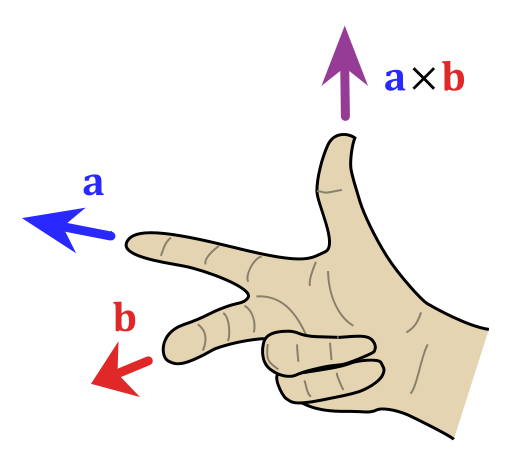
\includegraphics[width = 7cm]{cross right hand rule.png}
                    \caption{A diagram showing the right hand rule.\\Source: \href{https://commons.wikimedia.org/wiki/File:Right_hand_rule_cross_product.svg}{Acdx}, \CCSA}
                    \label{fig: cross product right hand rule}
                \end{figure}

                \begin{figure}[!h]
                    \centering
                    \begin{subfigure}[t]{0.45\textwidth}
                        \centering
                        \scalebox{0.9}
                        {
                            %trims left, bottom, right, top
                        \begin{adjustbox}{clip,trim=30mm 40mm 25mm 20mm}
                            {\import{images}{3D Cross Product Vector Diagram a.pgf}}
                        \end{adjustbox}
                        }
                    \end{subfigure}
                    \hfill
                    \begin{subfigure}[t]{0.45\textwidth}
                        \centering
                        \scalebox{0.6}
                        {
                            %trims left, bottom, right, top
                        \begin{adjustbox}{clip,trim=25mm 30mm 5mm 10mm}
                            {\import{images}{3D Cross Product Vector Diagram b.pgf}}
                        \end{adjustbox}
                        }
                    \end{subfigure}
                    \vspace{-8mm}
                    \caption{Diagrams showing the cross product of two vectors $\bvec{v}$ and $\bvec{u}$.}
                \end{figure}

                \newpage
                \subsubsection{Properties of the Cross Product}
                    \label{subsubsec: Properties of the Cross Product}

                    The cross product has some strange identities associated with it, primarily because it is not commutative or associative.

                    \begin{equation}
                        \vect{a} \times \vect{b} = -(\vect{b} \times \vect{a})
                    \end{equation}
                    \begin{equation}
                        \gamma (\vect{a} \times \vect{b}) = (\gamma\vect{a}) \times \vect{b} = \vect{a} \times (\gamma\vect{b})
                    \end{equation}
                    \begin{equation}
                        \vect{a} \times (\vect{b} + \vect{c}) = \vect{a} \times \vect{b} + \vect{a} \times \vect{c}
                    \end{equation}
                    \begin{equation}
                        \vect{a} \cdot (\vect{a} \times \vect{b}) = \vect{b} \cdot (\vect{a} \times \vect{b}) = 0
                    \end{equation}

                    You might recall that the area of a triangle with side lengths $a,\, b,\, c$ and opposite angles $A,\, B,\, C$ has an area $A = \frac{1}{2}ab\sin C$ (where $C$ is the angle between the sides $a$ and $b$).\\
                    We can instead look at \figref{fig: Dot Product Diagram} or \figref{fig: Area of Cross Product} and think of these sides as $\bvec{v}$ and $\bvec{u}$, with the angle between them as $\theta$.\\
                    By \eqref{eq: cross product magnitude} we then know that the magnitude of the cross product of these two vectors gives double the area of this triangle.
                    Therefore, the magnitude of the cross product gives \textit{double the area of the triangle} inscribed by the vectors or \textit{the area of the parallelogram} inscribed by the vectors (\figref{fig: Area of Cross Product}).

                    \begin{figure}[!h]
                        \centering
                        \begin{subfigure}[t]{0.45\textwidth}
                            \centering
                            \scalebox{0.65}
                            {
                                %trims left, bottom, right, top
                            \begin{adjustbox}{clip,trim=30mm 10mm 15mm 10mm}
                                {\import{images}{Cross Product Triangle Area.pgf}}
                            \end{adjustbox}
                            }
                        \end{subfigure}
                        \hfill
                        \begin{subfigure}[t]{0.45\textwidth}
                            \centering
                            \scalebox{0.65}
                            {
                                %trims left, bottom, right, top
                            \begin{adjustbox}{clip,trim=30mm 10mm 15mm 10mm}
                                {\import{images}{Cross Product Parallelogram Area.pgf}}
                            \end{adjustbox}
                            }
                        \end{subfigure}
                        \vspace{-5mm}
                        \caption{Diagrams showing areas of the triangle and parallelogram inscribed by vectors $\bvec{v}$ and $\bvec{u}$ and the relationship to the cross product of two.}
                        \label{fig: Area of Cross Product}
                    \end{figure}
        
                    \newpage

            \subsection{Some Useful Vector Identities}

                Here in this section we will simply sate some vector identities that can be rather tedious to prove.

                \begin{gather}
                    \vect{A}\cdot(\vect{B}\times\vect{C}) = \vect{B}\cdot(\vect{C}\times\vect{A}) = \vect{C}\cdot(\vect{A}\times\vect{B})\\
                    \vect{A}\times(\vect{B}\times\vect{C}) = (\vect{A}\cdot\vect{C})\vect{B} - (\vect{A}\cdot\vect{B})\vect{C}\\
                    (\vect{A}\times\vect{B})\cdot (\vect{C}\times\vect{D}) = (\vect{A}\cdot\vect{C})(\vect{B}\cdot\vect{D}) - (\vect{A}\cdot\vect{D})(\vect{B}\cdot\vect{C})
                \end{gather}
                    

            \newpage

            \section{Matrices}
                \subsection{Matrix Notations \& Definitions}

                A matrix is similar to a vector, but instead of being a column of numbers, it is a rectangle of numbers.

                Convention is to use uppercase letters to denote a matrix. To denote a matrix $A$ that is $m$ items tall and $n$ items across we write $A_{m \times n}$. The element in the $i^{\text{th}}$ row and $j^{\text{th}}$ column is written with the lowercase letter i.e. $a_{ij}$.

                We would write such a matrix as in \eqref{eq: General Matrix}

                \begin{equation}
                    A_{m \times n} = \Matrix{a_{11} & a_{12} & \cdots & a_{1n}\\
                                            a_{21} & a_{22} & \cdots & a_{2n}\\
                                            \vdots & \vdots & \ddots & \vdots\\
                                            a_{m1} & a_{m2} & \cdots & a_{mn}}
                    \label{eq: General Matrix}
                \end{equation}

                for example

                \begin{equation*}
                    A_{2 \times 3} = \Matrix{1 & 2 & 3\\
                                            4 & 5 & 6}
                \end{equation*}

                Sometimes to make it explicit that a variable is a matrix it will be written with square brackets around it i.e. $\mtrx{A}$.

                \subsubsection{Definitions}

                    A square matrix is a matrix of the form $A_{n \times n}$.

                    The $n$ identity matrix $I_n$ is a square matrix with width and height $n$ that has 1s along its diagonal and 0s in all other entries.

                    \begin{equation}
                        I_3 = \Matrix{1 & 0 & 0\\0 & 1 & 0\\0 & 0 & 1}
                        \label{eq: Identity Matrix Example}
                    \end{equation}

                \subsection{Multiplying a Matrix by a Scalar}

                    This works basically as one would expect. If you have a matrix $A_{m \times n}$ and multiply it by some scalar $\gamma$ then every element is multiplied by $\gamma$.

                    For example

                    \begin{equation*}
                        3 A = 3 \Matrix{1 & 2 & 3\\4 & 5 & 6} = \Matrix{3 & 6 & 9\\12 & 15 & 18}
                    \end{equation*}

                \subsection{Matrix Addition}

                    To add two matrices together they must be of the same dimension (i.e. both must be $m \times n$ where $m$ and $n$ are the same for both matrices).

                \subsection{Matrix Multiplication}
                    \label{subsec: Matrix Multiplication}

                    Multiplying two matrices together is far more complex than one would expect. It is very different to addition in that here the operation is not done component-wise.

                    We begin by setting some rules:
                    \vspace{-1em}
                    \begin{itemize}
                        \item To multiply two matrices together $A$ and $B$, $B$ must have the same number of rows as $A$ has columns i.e. the matrices must be of the form $A_{m \times n}B_{n \times k}$
                        \item The multiplication is not commutative (i.e. $AB \neq BA$), in fact, the multiplication of $A$ and $B$ in reverse order from above (i.e.$B_{n \times k}A_{m \times n}$) is not allowed unless $k = m$.
                        \item Multiplication of the form $A_{m \times n}B_{n \times k}$ gives a third matrix $C_{m \times k}$.
                    \end{itemize}

                
                    Take the multiplication of the two matrices $A$ and $B$ produces a matrix $C$ of the form \\$A_{m \times n}B_{n \times k} = C_{m \times k}$.

                    To find the $ij^{\text{th}}$ term of $C$ you, for lack of a better explanation, take the dot product of the $i^{\text{th}}$ row of $A$ with the $j^{\text{th}}$ column of $B$.

                    For example:

                    \begin{equation*}
                        A_{3 \times 2}B_{2 \times 3} = C_{3 \times 3}
                    \end{equation*}
                    \begin{equation*}
                        \Matrix{a_{11} & a_{12}\\a_{21} & a_{22}\\a_{31} & a_{32}}\Matrix{b_{11} & b_{12} & b_{13}\\b_{21} & b_{22} & b_{23}} = \Matrix{(a_{11}b_{11} + a_{12}b_{21}) & (a_{11}b_{12} + a_{12}b_{22}) & (a_{11}b_{13} + a_{12}b_{23})\\[0.5em] (a_{21}b_{11} + a_{22}b_{21}) & (a_{21}b_{12} + a_{22}b_{22}) & (a_{21}b_{13} + a_{22}b_{23}) \\[0.5em] (a_{31}b_{11} + a_{32}b_{21}) & (a_{31}b_{12} + a_{32}b_{22}) & (a_{31}b_{13} + a_{32}b_{23})}
                    \end{equation*}
                    \begin{equation*}
                        \Matrix{1 & 2\\3 & 4\\5 & 6}\Matrix{2 & 4 & 6\\8 & 10 & 12} = \Matrix{((1)(2) + (2)(8)) & ((1)(4) + (2)(10)) & ((1)(6) + (2)(12))\\[0.5em] ((3)(2) + (4)(8)) & ((3)(4) + (4)(10)) & ((3)(6) + (4)(12)) \\[0.5em] ((5)(2) + (6)(8)) & ((5)(4) + (6)(10)) & ((5)(6) + (6)(12))} = \Matrix{18 & 24 & 30\\ 38 & 52 & 66\\ 58 & 80 & 102}
                    \end{equation*}

                    Left multiplication of an $m \times n$ matrix by $I_m$ (\eqref{eq: Identity Matrix Example}) or right multiplication by $I_n$ is equivalent to multiplying by 1.

                    \begin{equation}
                        I_m A_{m \times n} = A_{m \times n} I_n = A_{m \times n}
                    \end{equation}

                
                \newpage

                \subsection{Matrix Transposes}
                    
                    The transpose of a matrix $A$ is denoted by $A^T$.

                    To get the transpose of $A$ the $n^{\text{th}}$ row of $A$ becomes the $n^{\text{th}}$ column of $A^T$ (or the $n^{\text{th}}$ column of $A$ becomes the $n^{\text{th}}$ row of $A^T$, either works).

                    The easiest way to remember this is `\textit{Rows to columns, columns to rows.}'
                    
                    For example:
                    \begin{equation*}
                        \left(\Matrix{1 & 2 & 3\\ 4 & 5 & 6}\right)^T = \Matrix{1 & 4\\ 2& 5\\ 3 & 6}
                    \end{equation*}

                \subsection{Determinants}

                    The determinant of a square matrix $A$ is denoted either by $\text{det}(A)$ or $|A|$.

                    Take an $n \times n$ matrix $A$. To use the formula for the determinant one must first make an arbitrary choice of either $1 \leq i \leq n$ or $1 \leq j \leq n$.

                    \subsubsection{Some Required Notation}
                    We denote a matrix $A_{ij}$ as the matrix $A$ with the $i^{\text{th}}$ row and $j^{\text{th}}$ column removed.

                    For example

                    \begin{equation*}
                        A = \Matrix{1 & 2 & 3\\4 & 5 & 6\\7 & 8 & 9} \Rightarrow A_{22} = \Matrix{1 & 3\\7 & 9}
                    \end{equation*}

                    \subsubsection{The formulas}
                    If an arbitrary $i$ was chosen then the formula is iterated through all $j$:

                    \begin{equation}
                        |A| \deq \sum_{j = 1}^n (-1)^{i + j}\,a_{ij}\,|A_{ij}|
                    \end{equation}

                    For an arbitrary $j$ then the formula is iterated through all $i$:

                    \begin{equation}
                        |A| \deq \sum_{i = 1}^n (-1)^{i + j}\,a_{ij}\,|A_{ij}|
                    \end{equation}

                    This formula is a rare example of a recursive formula, in that to define the determinant for an $n \times n$ matrix you need to know how to find the determinant of a $(n-1) \times (n-1)$ matrix.\\
                    It is worth noting that we define the determinant of a $1\times 1$ matrix as just the number (i.e. the determinant of the matrix $[x]$ is $x$.)\\
                    Therefore this formula can then be used to define the determinant of a $2 \times 2$ matrix using this definition, then the $2 \times 2$ for a $3 \times 3$ etc.


                \subsection{Matrix Inversion}

                    While you cannot divide by a matrix, in some cases you can multiply by another matrix which cancels out a matrix. This is called matrix inversion and the inverse of a matrix is denoted by a $-1$ power i.e. $A^{-1}$.\\
                    For a matrix to be invertible it \textbf{must} be a square matrix. A square matrix does not always have an inverse, but if it does then the following is true.

                    Let $A$ be an $n \times n$ matrix that has an inverse:
                    \begin{equation}
                        A^{-1}A = AA^{-1} = I_n
                    \end{equation}


                    There are many conditions that can be used to determine whether a matrix is invertible, but perhaps the simplest is the requirement that the determinant be non 0 (i.e. $|A| \neq 0$).

                    Provided this condition is met, the inverse is given by \eqref{eq: Matrix Inverse}.

                    \begin{equation}
                        A^{-1} = \frac{1}{|A|}\left(C_{ij}\right)^T
                        \label{eq: Matrix Inverse}
                    \end{equation}

                    Here $C_{ij}$ is the matrix where every $ij^{\text{th}}$ element $c_{ij}$ of the matrix is given by

                    \begin{equation}
                        c_{ij} = (-1)^{i+j}|A_{ij}|
                    \end{equation}

                    Where $A_{ij}$ is $A$ with the $i^{\text{th}}$ row and $j^{\text{th}}$ column removed.

                    If a matrix is invertible then there is the identity that $|A^{-1}| = \bfrac{1}{|A|}$


                    

\end{document}